\documentclass[
  aps,
  reprint,
  superscriptaddress,
  floatfix,
  nofootinbib,
  longbibliography
]{revtex4-2}

\usepackage{amsmath,amssymb}
\usepackage{graphicx}
\usepackage{xcolor}
\usepackage{tikz}
\usetikzlibrary{calc,positioning,arrows.meta}
\usepackage{hyperref}

\hypersetup{
  colorlinks=true,
  linkcolor=blue,
  citecolor=blue,
  urlcolor=blue
}

% --- convenience macros -------------------------------------------------
\newcommand{\R}{\mathbb{R}}
\newcommand{\E}{\mathbb{E}}
\newcommand{\Prob}{\mathbb{P}}
\newcommand{\Sph}[1]{S^{#1}}
\newcommand{\Nq}{N_{\mathrm q}}
\newcommand{\sint}{\sigma_{\mathrm{int}}}
\newcommand{\Eint}{E_{\mathrm{int}}}
\newcommand{\T}{^{\mathsf{T}}}
\newcommand{\opnorm}[1]{\lVert #1 \rVert_{\mathrm{op}}}
\newcommand{\norm}[1]{\lVert #1 \rVert}
\newcommand{\ReLU}{\mathrm{ReLU}}

\DeclareMathOperator*{\argmax}{arg\,max}
\DeclareMathOperator{\spanop}{span}
\DeclareMathOperator{\Var}{Var}

\begin{document}

\title{Geometric Limits on Semantic Expressibility: Quantum-Inspired Contexts and Polysemy in Large Language Models}

\author{Karl Svozil}
\email{karl.svozil@tuwien.ac.at}
\affiliation{Institute for Theoretical Physics, TU Wien,
Wiedner Hauptstra\ss{}e 8--10/136, 1040 Vienna, Austria}

\date{\today}

\begin{abstract}
The geometric argument uses two counts.  The \emph{exact dimension} $d$ is
the number of mutually orthogonal axes in the usable representation space.
The \emph{quasi-dimensional count} $\Nq$ is the number of semantic directions
represented with small, but nonzero, mutual overlap.  Useful
quasi-dimensionality lies between two failures.  If $\Nq\leq d$, exact
orthogonal axes remain available and overcomplete encoding is unnecessary.
If $\Nq$ is too large, the largest pairwise overlaps become too strong.  For
random-like directions and tolerated overlap $\varepsilon$, the resulting
Goldilocks estimate is
\[
       d<\Nq\lesssim \exp(d\varepsilon^2/4).
\]
Only a subset of size $k$ is active at once; its readout interference scales
as $\sqrt{k/d}$.  Here $\varepsilon$ and $k$ are controls, not additional
dimensions.  On this geometric foundation we give a quantum-inspired but
classically implementable model of polysemy: context observables share a
token-associated spectral projector while acting differently, and generically
noncommutatively, on sense subspaces in its orthogonal complement. Conditional
projection onto a selected observable supplies a contextual embedding.  The
Goldilocks estimate and the intertwined-observable construction are separately
testable and require no claim of physical quantum computation.
\end{abstract}

\maketitle


% ======================================================================
\section{Introduction}
\label{sec:intro}
% ======================================================================

This chapter examines contextual representation in large language models
(LLMs) as part of the volume's broader inquiry into ``quantum thinking.''
Only a minimal orientation to LLM operation is needed here.  Input text is
first divided into tokens, and each token is mapped to an initial vector.
Transformer blocks then use self-attention and feed-forward transformations
to turn those initially context-free vectors into sequence-dependent hidden
states.  An output layer converts the final state into token scores, and a
softmax distribution supports probabilistic next-token selection.  This
compact chain---tokens, embeddings, contextual transformation, and finite
readout---supplies the computational background for the argument below; the
details of pre-training, fine-tuning, reinforcement learning, and
backpropagation are not required.

Current Transformer-based LLMs are classical computational systems.  They
run on classical hardware and use real-valued matrix operations,
normalization, nonlinearities, copying, and generally irreversible updates.
Their reliance on vectors, inner products, high dimension, or probabilistic
output does not by itself make them quantum or even quantum-like.  The more
limited question pursued here is where ordinary high-dimensional geometry
already explains the coexistence and contextual selection of semantic
features, and where a stronger comparison with quantum-like formalisms might
begin.  Such a comparison would have to do more than rename familiar neural
operations: it would need to identify a role for contextual bases or subspaces,
incompatible or noncommuting alternatives, interference, or
measurement-like readout that yields explanatory or predictive value beyond
a classical dynamic-embedding account.

Semantic concurrency makes this boundary concrete.  A model must preserve
many latent possibilities while making only a small, context-selected subset
operationally accessible.  Polysemy is the simplest illustration: the same
token can participate in financial, river-edge, or seat/bench contexts of
``bank,'' yet the surrounding sequence drives it toward different contextual
representations.  The verb in an aircraft ``banks'' supplies a fourth sense,
mentioned below but not used in the three-arm schematic.  This relation among
possibility, context, and readout
connects directly to the volume's recurring themes without implying that the
underlying machine is physically quantum.  It also motivates a separation
between what a representation can geometrically accommodate and what a
finite channel can reliably recover.



The claims below occupy different rungs of that evidential
ladder.  Concentration of measure and exponential packing are standard
results of high-dimensional geometry.  Their use to describe semantic
capacity, together with the accumulated-interference estimate, is a formal
model of classical representation subject to stated assumptions about the
usable carrier and coactivation.  The reference-subspace organization is
a stronger empirical hypothesis about LLM internals and is tested against
classical controls.  The comparison with quantum contextuality remains a
limited structural correspondence; no physical quantumness, Born-rule
dynamics, or semantic Kochen--Specker theorem is inferred.

A finite-dimensional activation space faces a two-sided tension.  The exact
dimension $d$ is the number of mutually orthogonal axes available in the
usable carrier.  The second count, $\Nq$, is the number of semantic directions
treated as quasi-dimensions.  If $\Nq\leq d$, exact orthogonality remains
available.  Once $\Nq>d$, the code is overcomplete and quasi-orthogonality
becomes useful.  Yet increasing $\Nq$ still further eventually produces too
many large pairwise overlaps.  This is the Goldilocks zone between an
underloaded exact-axis regime and an overcrowded quasi-dimensional regime.

The two sides obey different scalings. On the capacity side,
concentration of measure permits exponentially many candidate semantic
directions with pairwise overlap at most $\varepsilon$,
%
\begin{equation}
\label{eq:intro-capacity}
\Nq\lesssim \exp(d\varepsilon^{2}/4).
\end{equation}
%
On the readout side, the same small residual overlaps add in quadrature
over an active set of size $k$, giving an interference scale
%
\begin{equation}
\label{eq:intro-readout}
\sint\sim\sqrt{k/d}.
\end{equation}
%
The first relation estimates how many quasi-dimensions fit into $d$ exact
dimensions at overlap tolerance $\varepsilon$.  The second estimates the
readout noise when $k$ of them are active.  Neither $\varepsilon$ nor $k$ is
another dimension: $\varepsilon$ is an overlap tolerance and $k$ is an active
count.  Together the relations make $d$ a \emph{semantic concurrency
bandwidth}.

Polysemy is the cleanest example. A single lexical item, such as
``bank'', can access several mutually exclusive meanings, only one of
which is selected in a given context. The same tension appears more
generally in feature superposition, role binding, and compositional
semantics~\cite{mikolov2013}: many latent semantic degrees of freedom
must coexist, while only a context-selected subset is read out. We use
polysemy as a controlled entry point because it makes contextual
selection explicit. In lexical semantics, polysemy is distinguished
from homonymy by the relatedness of senses~\cite{pustejovsky1995}.
Modern Transformer-based LLMs implement contextual selection through
dynamic contextual embeddings: a token representation is repeatedly
transformed by self-attention and MLP layers as it absorbs information
from its sentential environment~\cite{Vaswani-2017-Attention}.

The chapter develops two central ideas.  First, concentration permits a large
semantic dictionary, but both dictionary crowding and accumulated
interference delimit a quantitative Goldilocks bracket.  This geometric claim
is architecture-independent once $d$, $\Nq$, the overlap tolerance
$\varepsilon$, and the active count $k$ have been operationally defined.
Second, for some canonically
polysemous tokens, contexts may be represented by intertwined symmetric
operators.  These operators share a stable token-associated spectral
projector, while sense information occupies low-dimensional subspaces in its
orthogonal complement.  Selecting or mixing the corresponding conditional
projections implements a contextual embedding.  This operator construction
is not implied by concentration geometry; it is a stronger empirical model,
and Sec.~\ref{sec:predictions} states how it can fail.

A serious caveat is anisotropy.  The nominal width of an LLM layer may exceed
the dimension of the carrier actually occupied by its states.  To avoid a
third dimensional symbol, $d$ throughout this chapter means the \emph{usable
exact dimension}: first restrict or whiten the representation to the carrier
being tested, then let $d$ be the size of an orthonormal basis of that carrier.
If this usable $d$ is small, the quasi-dimensional capacity weakens.  The
method used to identify the carrier must therefore be declared empirically.

The reference-subspace and operator hypotheses have a narrower domain. They
are meant for
canonically polysemous tokens with established sense inventories, such
as WordNet-, OntoNotes-, SemCor-, or WiC-style sense
distinctions~\cite{pilehvar2019wic} with enough contextual instances
for testing. Failure on a representative sample, against the controls in
Sec.~\ref{sec:predictions}, would count against a privileged token reference
direction or an intertwined-observable implementation even if the broader
Goldilocks capacity/accessibility picture survives.

The proposal is adjacent to the superposition hypothesis in mechanistic
interpretability~\cite{elhage2022superposition}, according to which neural networks
represent more features than they have neurons by packing features into
nearly orthogonal directions. The present chapter separates the
geometric background from a possible semantic organization within it.
The general superposition picture concerns an overcomplete dictionary
of feature directions and sparse active sets. The present model adds the more
specific possibility that contextual readout is organized around stable
token-associated directions and context-dependent, potentially noncommuting
projectors.

Section~\ref{sec:concentration} develops the capacity framework:
quasi-orthogonality, L\'evy's lemma, exponential packing, and the
kinetic/epistemic distinction, culminating in the Goldilocks bracket of
Sec.~\ref{sec:goldilocks}. Section~\ref{sec:reference} introduces the
reference-subspace hypothesis, its realization by intertwined context
observables, and its relation to dynamic contextual embeddings.
Section~\ref{sec:attention} connects the construction to attention as soft
context routing rather than literal basis reconstruction.
Section~\ref{sec:discussion} discusses superposition, sparse
autoencoders, limitations, empirical tests, and the limited quantum
analogy.

{The two dimensional counts.}
Throughout, $\R^{d}$ is the usable Euclidean carrier.  Its exact dimension
$d$ is the size of any orthonormal basis.  The symbol $\Nq$ denotes the number
of approximately orthogonal semantic directions represented in that carrier;
these are the paper's \emph{quasi-dimensions}.  Thus $\Nq$ is a count of
directions, not the dimension of a second vector space.  Other symbols are
controls or local ranks: $\varepsilon$ is an overlap tolerance, $k$ is the
number simultaneously active, and the later $p$ and $q_C$ count basis vectors
inside particular reference and sense subspaces.

The carrier has inner product $u\T v$
and norm $\norm{v}=\sqrt{v\T v}$; $\Sph{d-1}=\{v\in\R^{d}:\norm{v}=1\}$
is the unit sphere; $I$ is the identity matrix; $\opnorm{\cdot}$ is the
operator norm; $A\succeq0$ means positive semidefinite; and $\Prob$ and
$\E$ denote probability and expectation under the uniform measure on
the relevant sphere unless stated otherwise. Universal positive
constants are denoted $c,c'$, possibly changing from line to line.

% ======================================================================
\section{Concentration geometry and capacity}
\label{sec:concentration}
% ======================================================================

This section is architecture-independent. It gives the geometric
capacity constraint on which the later reference-subspace hypothesis builds.

\subsection{Quasi-orthogonality}
\label{sec:quasiortho}

Let $w_{1},\dots,w_{\Nq}\in\R^{d}$ be unit semantic directions. Strict
orthogonality, $w_i\T w_j=0$ for $i\neq j$, allows at most $\Nq=d$ such
vectors. Semantic
encoding does not require exact orthogonality. It requires approximate
distinguishability. We therefore call a family
$\varepsilon$-quasi-orthogonal if
%
\begin{equation}
\label{eq:quasiortho}
|w_i\T w_j|\le \varepsilon,\qquad i\neq j .
\end{equation}
%
We use ``quasi-orthogonal'' rather than ``pseudo-orthogonal'': the latter is
normally reserved for geometry with an indefinite inner product, which is not
intended here.

This is the relevant notion for high-dimensional feature storage:
small overlap is tolerable, provided readout can absorb the resulting
interference.

\subsection{L\'evy's lemma and linear overlaps}
\label{sec:levy}

High-dimensional spheres make quasi-orthogonality generic.

%\paragraph*{Heuristic concentration argument.}
The mechanism is already visible before invoking the formal lemma.  Let
\[
        x=(x_1,\ldots,x_d)\in\R^d
\]
be a unit vector chosen without a preferred direction.  Then
\[
        x_1^2+\cdots+x_d^2=1 .
\]
Rotational invariance suggests that the norm is spread over the available
coordinates, so a typical coordinate weight is of order $1/d$.  Now fix a
unit direction $u$.  By rotational invariance one may choose coordinates so
that $u=e_1$.  The squared overlap with the random direction is then
\[
        |u\T x|^2=x_1^2 .
\]
Thus the overlap with any fixed direction is typically of order $d^{-1/2}$
in amplitude, or $1/d$ in squared amplitude.  A macroscopic overlap
$|u\T x|>\varepsilon$ therefore requires one coordinate to carry an
anomalously large fraction of the total norm.  In high dimension such an
event is exponentially unlikely.

The same intuition appears particularly transparently in a $d$-dimensional
complex Hilbert-space analogue.  If $\psi\in\mathbb{C}^d$ is Haar-random and
$\phi$ is fixed, unitary invariance permits the choice $\phi=e_1$, so
\[
        |\langle\phi,\psi\rangle|^2=|\psi_1|^2 .
\]
For a Haar-random complex unit vector the exact tail is
\[
        \Prob\{ |\langle\phi,\psi\rangle|^2\geq\eta\}
        =(1-\eta)^{d-1}
        \leq \exp[-(d-1)\eta] .
\]
For real embedding vectors the analogous spherical concentration estimate
has the operative scaling
\[
        \Prob\{ |u\T x|>\varepsilon\}
        \lesssim \exp(-c d\varepsilon^2)
\]
for a universal constant $c>0$.  Consequently, if $\Nq$ random directions are
sampled, a union-bound estimate gives a probability at most of order
$\Nq^2\exp(-c d\varepsilon^2)$ that some pair has overlap larger than
$\varepsilon$.  Hence $\Nq$ may grow exponentially in $d\varepsilon^2$ while
all pairwise overlaps remain small with high probability.  This is the
heuristic core of the exponential quasi-orthogonal capacity derived below.

L\'evy's lemma makes this intuition precise.  If $f:\Sph{d-1}\to\R$
is $L$-Lipschitz, then
%
\begin{equation}
\label{eq:levy}
\Prob\bigl(|f(v)-\E f|\ge\delta\bigr)
 \le
2\exp\!\left(-\frac{c\,d\,\delta^{2}}{L^{2}}\right),
\end{equation}
%
for a universal $c>0$~\cite{ledoux2001concentration,milman1986asymptotic}. Apply this to the
linear functional $f_u(v)=u\T v$. It is $1$-Lipschitz and has mean zero
by symmetry. Hence
%
\begin{equation}
\label{eq:overlap}
\Prob\bigl(|u\T v|\ge\varepsilon\bigr)
 \le 2\exp(-c\,d\,\varepsilon^{2}).
\end{equation}
%
For normalized surface measure one obtains the explicit form
$2\exp(-(d-1)\varepsilon^{2}/2)$~\cite{ledoux2001concentration}. Thus two random
unit vectors are nearly orthogonal with high probability, and typical
overlap amplitudes scale as $d^{-1/2}$.

In trained models, $d$ means the usable carrier defined in the Introduction,
not automatically the nominal layer width.  Anisotropy or a narrow activation
cone requires restriction or whitening before the orthonormal-basis size $d$
is assigned.

{Relation to Johnson--Lindenstrauss.}
The Johnson--Lindenstrauss lemma preserves pairwise distances among
$n$ points after projection to dimension
$r=O(\varepsilon^{-2}\log n)$~\cite{johnson-1984}. Here $r$ is only the
temporary target rank in that theorem; it is unrelated to the active-set
count $k$ used below. The lemma is driven by the
same concentration phenomenon as Eq.~\eqref{eq:overlap}; indeed JL can
be derived from sphere concentration applied to projection
norms~\cite{Dasgupta-2003}. Here L\'evy's lemma is the more direct tool:
the issue is not projecting a finite dataset, but the typical overlap
between semantic directions in the representation space.

\subsection{Exponential packing}
\label{sec:packing}

Sample $\Nq$ unit vectors independently and uniformly from
$\Sph{d-1}$. By Eq.~\eqref{eq:overlap} and a union bound over pairs,
%
\begin{equation}
\label{eq:unionbound}
\Prob\bigl(\exists\,i\neq j:\ |w_i\T w_j|\ge\varepsilon\bigr)
 < \Nq^{2}\exp(-c\,d\,\varepsilon^{2}).
\end{equation}
%
This probability is below one, and hence an
$\varepsilon$-quasi-orthogonal family exists, provided
%
\begin{equation}
\label{eq:packing}
\Nq < \exp\!\left(\frac{c}{2}\,d\,\varepsilon^{2}\right).
\end{equation}
%
This is the kinetic capacity estimate: for large usable exact dimension $d$,
many candidate semantic directions can coexist with small pairwise
overlap.

The estimate controls pairwise overlap only. It does not guarantee that
a large collection of feature directions is well-conditioned. By Gershgorin,
$|w_i\T w_j|\le\varepsilon$ gives only
$\opnorm{G-I}\le(n-1)\varepsilon$ for an $n$-element Gram matrix, which
is useless when $n$ is large. Joint readout therefore needs a
separate conditioning assumption, introduced in Sec.~\ref{sec:gated}.

\subsection{Kinetic capacity versus epistemic accessibility}
\label{sec:kinetic-epistemic}

The packing bound says what can coexist. It does not say what can be
read. We call the coexistence supply \emph{kinetic semantic capacity}.
We call the recoverable subset \emph{epistemic semantic accessibility}.
The distinction is the central point of the chapter.

Let $\Nq$ candidate features be represented by unit directions
$w_1,\dots,w_{\Nq}\in\R^{d}$. In a given context, suppose an active set
$S$ of size $k$ contributes amplitudes $x_j$, producing
%
\begin{equation}
\label{eq:hidden}
h=\sum_{j\in S}x_j w_j .
\end{equation}
%
A linear readout of feature $i$ gives
%
\begin{equation}
\label{eq:readout}
w_i\T h
=
x_i+
\sum_{\substack{j\in S\\ j\neq i}}
x_j\,w_i\T w_j .
\end{equation}
%
The first term is signal; the second is interference. For random
incoherent directions,
%
\begin{equation}
\label{eq:moments}
\E[w_i\T w_j]=0,
\qquad
\Var(w_i\T w_j)\simeq \frac{1}{d}.
\end{equation}
%
Thus, conditional on the active amplitudes,
%
\begin{equation}
\label{eq:intvar}
\Var\!\left(
\sum_{\substack{j\in S\\ j\neq i}}
x_j\,w_i\T w_j
\right)
\simeq
\frac{1}{d}
\sum_{\substack{j\in S\\ j\neq i}}x_j^2 .
\end{equation}
%
For amplitudes of order unity,
%
\begin{equation}
\label{eq:sint}
\sint\sim\sqrt{\frac{k}{d}} .
\end{equation}
%
This is the readout bottleneck. Concentration lets many directions
coexist because their overlaps are small. But readout sees the
\emph{sum} of many small overlaps. Reliable recovery requires
%
\begin{equation}
\label{eq:snr}
\sqrt{\frac{k}{d}}\ll \Delta,
\end{equation}
%
where $\Delta$ is the relevant decision margin. Equivalently,
%
\begin{equation}
\label{eq:dual}
\text{kinetic: }\Nq\lesssim\exp(c\,d\,\varepsilon^{2}),
\qquad
\text{epistemic: }k\lesssim d\,\Delta^{2}.
\end{equation}
%
The first is storage-like coexistence. The second is simultaneous
accessibility. A model may host many more features than it can jointly
read.

\subsection{The Goldilocks zone in plain terms}
\label{sec:goldilocks}

Only two global geometric counts are needed.  The exact dimension $d$ is the
number of vectors in an orthonormal basis of the chosen usable carrier.  The
quasi-dimensional count $\Nq$ is the number of semantic directions represented
in that carrier.  Strictly speaking, $\Nq$ is a dictionary size rather than the
dimension of a second vector space.  We nevertheless call its members
``quasi-dimensions'' when their mutual overlaps are small enough for the
intended readout.  Any strong anisotropy or unused coordinates must be handled
when the usable carrier is chosen, before $d$ is assigned; it does not introduce
a third dimension symbol.

The three regimes can then be stated directly.  If $\Nq\leq d$, an exactly
orthogonal assignment is geometrically possible, although learning need not
select one and no semantic basis is privileged.  If $\Nq>d$, exact mutual
orthogonality is impossible, but many approximately orthogonal directions may
still coexist.  Eventually the dictionary becomes so crowded that some
directions overlap too strongly to remain reliably distinguishable.

A simple random-code estimate locates this transition.  For $\Nq$ random-like
unit directions in $\R^d$, the largest pairwise overlap is typically of order
%
\begin{equation}
\label{eq:max-overlap}
\mu_{\max}
:=\max_{i\ne j}|w_i\T w_j|
\approx 2\sqrt{\frac{\log \Nq}{d}}.
\end{equation}
%
The factor $2$ reflects the fact that a dictionary contains of order
$\Nq^2$ pairs.  If $\varepsilon$ is the largest acceptable overlap, solving
$\mu_{\max}\lesssim\varepsilon$ gives the transparent Goldilocks estimate
%
\begin{equation}
\label{eq:gold-simple}
\boxed{
d<\Nq\ \lesssim\ \exp\!\left(\frac{d\varepsilon^2}{4}\right)
}.
\end{equation}
%
The left boundary marks the onset of overcompleteness.  The right boundary
marks crowding under an isotropic random null model.  There is no unique
numerical upper boundary unless an overlap tolerance is chosen:
$\varepsilon$ is a distinguishability criterion, not another dimension.
Equivalently, supporting a prescribed quasi-dimensional count requires roughly
%
\begin{equation}
\label{eq:d-needed}
d\gtrsim\frac{4\log\Nq}{\varepsilon^2}.
\end{equation}

For example, let $d=4096$.  A single random pair then overlaps by about
$1/\sqrt d=1.6\%$ on its natural scale.  But $\Nq=10^4$ directions make almost
fifty million pairs, so Eq.~\eqref{eq:max-overlap} estimates the largest overlap
as about $9.5\%$.  With a $10\%$ tolerance, Eq.~\eqref{eq:gold-simple} gives the
illustrative band
%
\begin{equation}
\label{eq:gold-example}
4096<\Nq\lesssim 2.8\times10^4.
\end{equation}
%
This number is not an LLM constant.  It changes exponentially with the chosen
tolerance, and learned directions are neither independent nor isotropic.

Simultaneous accessibility is a separate issue.  If $k$ directions are active
at once, their residual interference has the scale
$\sint\sim\sqrt{k/d}$ from Eq.~\eqref{eq:sint}.  Here $k$ is an active-set count,
not a dimension.  For $d=4096$ and $k=64$, the null-model interference scale is
$0.125$.  Thus a dictionary can lie inside the geometric Goldilocks zone yet
still be difficult to read when too many of its directions are activated
together.

Figure~\ref{fig:toy-scalings} illustrates these two statements.  It is not a
model of a trained language model, but a null model for concentration geometry.
Departures in trained representations would be informative about anisotropy,
learned feature alignment, nonlinear readout, or coactivation-dependent
orthogonalization.

\begin{figure*}[t]
\centering
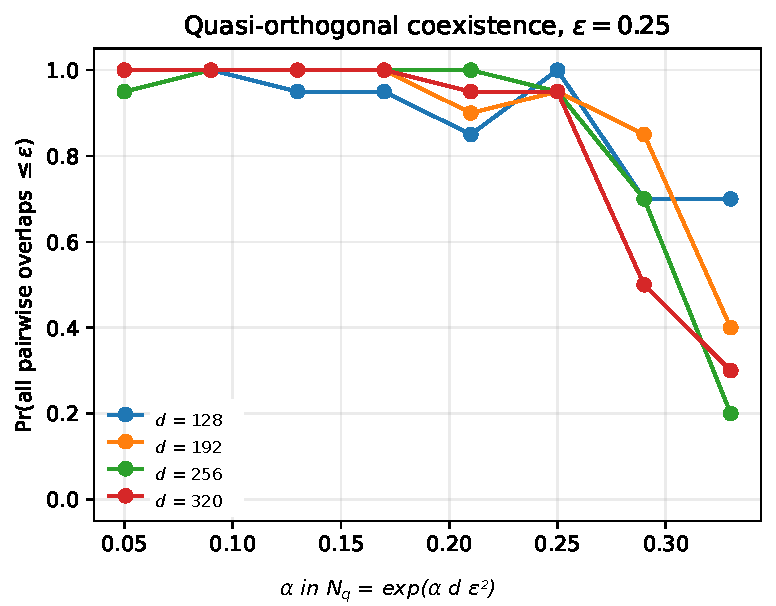
\includegraphics[width=0.48\textwidth]{2026-llm-quasi_orthogonal_coexistence.pdf}
\hfill
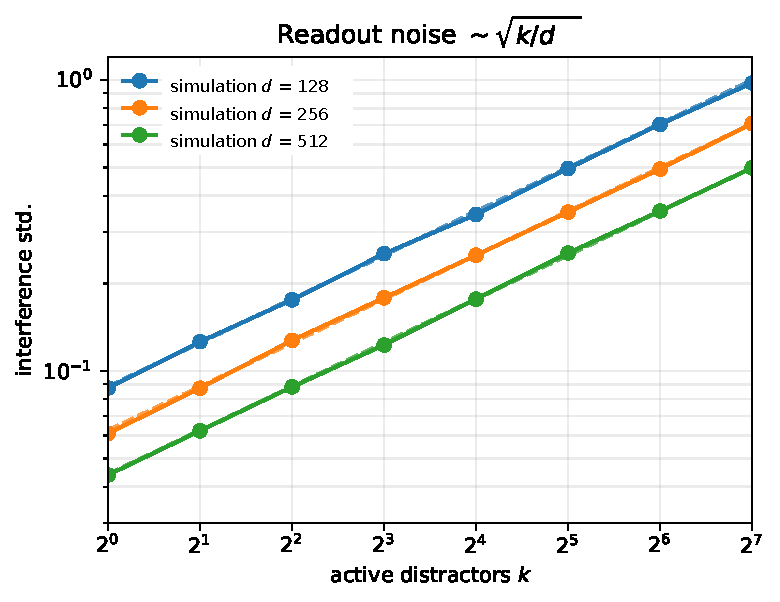
\includegraphics[width=0.48\textwidth]{2026-llm-readout_interference.pdf}
\caption{%
Synthetic geometry checks for the capacity/accessibility distinction.
Left: random unit directions in exact usable dimension $d$ are sampled with
$\Nq=\exp(\alpha d\varepsilon^{2})$ and tested for
$\varepsilon$-quasi-orthogonality. For sufficiently small $\alpha$,
large families coexist with high probability, illustrating the
exponential packing side of Eq.~\eqref{eq:dual}. Right: for a fixed
target direction, $k$ random distractor directions are simultaneously
active with random signs. The standard deviation of the readout
interference follows the predicted scale
$\sint\sim\sqrt{k/d}$, illustrating the accessibility side of
Eq.~\eqref{eq:dual}. Together the panels visualize coexistence and
simultaneous accessibility. Both use random isotropic vectors and should
be read as a geometric null model rather than as measurements on a
trained language model.
}
\label{fig:toy-scalings}
\end{figure*}

This also clarifies the relation to compressed sensing.  A dictionary of
$\Nq$ feature directions with only $k$ active at once can sometimes be read
from far fewer than $\Nq$ coordinates.  Under suitable incoherence or
restricted-isometry assumptions, the familiar scaling is
$d\gtrsim Ck\log(\Nq/k)$~\cite{donoho2006compressed,candes2006robust,foucart2013mathematical}.
The analogy is diagnostic rather than literal: hidden states are anisotropic,
feature activation is structured, and transformer readout is nonlinear.

% ======================================================================
\section{Token reference subspaces and intertwined context observables}
\label{sec:reference}
% ======================================================================

The previous section established an architecture-independent capacity
constraint. We now ask a more speculative question: does a trained model
organize the contextual states of some polysemous tokens relative to a
stable token-associated reference subspace? This hypothesis is not implied
by concentration geometry, and it is separately falsifiable.

The notation distinguishes mathematical types and roles. For a token $t$
and a sense context $C$:
%
\begin{itemize}
\item $r_t\in\R^d$ is a unit candidate token reference vector;
\item $\mathcal R_t\subset\R^d$ is the token reference subspace;
\item $P_t$ is the orthogonal projector onto $\mathcal R_t$;
\item $S_{t,C}\subset\mathcal R_t^\perp$ is a low-dimensional sense
subspace;
\item $u_{t,C,j}\in S_{t,C}$ are vectors spanning that sense subspace;
\item $h_\ell(t\mid x)\in\R^d$ is an observed contextual hidden state.
\end{itemize}
%
Thus $r_t$, $u_{t,C,j}$, and $h_\ell(t\mid x)$ are vectors, whereas
$\mathcal R_t$ and $S_{t,C}$ are subspaces. The $w_i$ used in
Sec.~\ref{sec:concentration} have a separate role: they are generic feature
directions in the capacity calculation and are not reused as sense labels.

\subsection{The reference-subspace hypothesis}
\label{sec:reference-hypothesis}

In the simplest version, let $r_t$ be a candidate unit direction and set
%
\begin{equation}
\label{eq:reference-direction}
\mathcal R_t=\spanop\{r_t\}.
\end{equation}
%
Empirically, $r_t$ could be the normalized static input embedding, a
normalized mean contextual embedding, or a learned token-specific probe
direction. It is simply a hypothesized context-stable reference for token
identity. It is not a mechanical or dynamical object.
Any state can be decomposed relative to any direction, so the decomposition
alone has no empirical content. The claim is that a token-associated
$\mathcal R_t$ exposes sense structure better than matched control
directions or subspaces.

For each context or sense label $C$, define a low-dimensional subspace
%
\begin{equation}
\label{eq:sense-subspace}
S_{t,C}=\spanop\{u_{t,C,1},\dots,u_{t,C,q_C}\}
\subset\mathcal R_t^\perp,
\qquad q_C\ll d .
\end{equation}
%
For the intended three-arm example, finance, river-edge, and seat/bench
associations of ``bank'' correspond to different subspaces
$S_{\mathrm{bank},C}$ inside the common orthogonal carrier
$\mathcal R_{\mathrm{bank}}^\perp$.  The verbal use in which an aircraft
banks or tilts supplies a fourth sense and would add a fourth context
subspace; it is mentioned here but omitted from the drawing for clarity.  A
word sense is not a single vector: topic, syntax, selectional preferences,
and world knowledge may require several spanning directions $u_{t,C,j}$.

The reference object may itself require more than one direction. In that
case define
%
\begin{equation}
\label{eq:reference-subspace}
\mathcal R_t=
\spanop\{r_{t,1},\dots,r_{t,p}\},
\qquad p\ge1,
\end{equation}
%
and require
%
\begin{equation}
\label{eq:multi-sense-subspace}
S_{t,C}\subset\mathcal R_t^\perp .
\end{equation}
%
Equation~\eqref{eq:reference-direction} is the special case $p=1$.
The bare subspace construction specifies only a pattern of sharing. In
quantum logic, different contexts can share one or more observables or
spectral projections; finite-dimensional examples with two shared
observables are known~\cite{svozil:040102}. In the semantic model,
$\mathcal R_t$ is a common token-associated reference subspace, while the
sense-specific subspaces lie in its orthogonal complement. These incidence
relations alone imply neither noncommutativity nor quantum probability. The
next subsection makes the stronger, optional operator structure explicit.

The low-rank assumption is empirical. It predicts that dominant
within-sense variation is low-dimensional after projection onto
$\mathcal R_t^\perp$. This is compatible with evidence that contextualized
embeddings can separate word senses, but it is stronger: it asks whether
such separation is privileged relative to a token-associated reference
subspace~\cite{wiedemann2019does,scarlini2020ares}.

\subsection{Intertwined context observables and conditional embeddings}
\label{sec:observables}

The shared-subspace idea can be implemented as a family of intertwined
context observables.  Let $Q_t\in\R^{d\times p}$ have orthonormal columns
spanning $\mathcal R_t$, so that $P_t=Q_tQ_t\T$.  For each context $C$, let
$B_{t,C}\in\R^{d\times q_C}$ have orthonormal columns spanning $S_{t,C}$.
Here $Q_t$ and $B_{t,C}$ are basis matrices, not semantic vectors.

The projector onto the token-plus-sense subspace is
%
\begin{equation}
\label{eq:context-projector}
\Pi_{t,C}=P_t+B_{t,C}B_{t,C}\T .
\end{equation}
%
All $\Pi_{t,C}$ contain the same spectral projector $P_t$ and therefore
intertwine on $\mathcal R_t$.  Their sense parts differ.  In particular,
%
\begin{equation}
\label{eq:projector-commutator}
[\Pi_{t,C},\Pi_{t,C'}]
=
[B_{t,C}B_{t,C}\T,B_{t,C'}B_{t,C'}\T]
\end{equation}
%
need not vanish.  Nonzero commutators represent incompatible conditional
decompositions: applying the two context projections in opposite orders can
give different intermediate states.

A symmetric context observable with this eigenspace structure is, for
example,
%
\begin{equation}
\label{eq:context-observable}
A_{t,C}
=Q_t\Lambda_tQ_t\T
 +B_{t,C}\Lambda_{t,C}B_{t,C}\T,
\end{equation}
%
where the diagonal matrix $\Lambda_t$ is shared across contexts and
$\Lambda_{t,C}$ is context-specific; their eigenvalue sets may be chosen
disjoint so that $P_t$ is identifiable as a shared spectral sector.  The operator acts as zero on the
unused orthogonal complement; an orthonormal completion may assign additional
eigenvalues without changing the shared structure.  With a nondegenerate
completed spectrum, $A_{t,C}$ is the real finite-dimensional analogue of a
maximal observable.  Generic choices for different $C$ need not commute,
although every $A_{t,C}$ retains the common spectral sector $P_t$.

The corresponding context-conditioned embedding is concrete:
%
\begin{equation}
\label{eq:observable-embedding}
h_{t,C}(x)
=\Pi_{t,C}h(x)
=P_t h(x)+B_{t,C}B_{t,C}\T(I-P_t)h(x).
\end{equation}
%
One may select a single $C$, or take a soft mixture of these embeddings as in
Sec.~\ref{sec:attention}.  Equations~\eqref{eq:context-projector}--
\eqref{eq:observable-embedding} provide the proposed implementation of
intertwining observables for contextual embedding.  They use ordinary real
matrices and can be trained or probed in a classical network.  Thus
noncommutativity here is a testable representational property, not evidence of
physical quantum dynamics or the Born rule.

\subsection{Projection and gated subspace readout}
\label{sec:gated}

Let $h(x)\in\R^d$ be a contextual state and retain the orthogonal projector
$P_t$ defined above. The two components are
%
\begin{align}
\label{eq:reference-decomp}
h(x)&=h_{\rm ref}(x)+h_\perp(x),\\
h_{\rm ref}(x)&=P_t h(x),\nonumber\\
h_\perp(x)&=(I-P_t)h(x)\in\mathcal R_t^\perp.\nonumber
\end{align}
%
For the one-dimensional case, $P_t=r_t r_t\T$ and the scalar
$a_t(x)=r_t\T h(x)$ measures the component along the reference direction.
The hypothesis is that most sense-disambiguating variation is present in
$h_\perp(x)$, not that the projection formula itself is special.

Readout inside $S_{t,C}$ also requires the spanning vectors to be
well-conditioned. Let
%
\begin{equation}
U_{t,C}=[\,u_{t,C,1}\ \cdots\ u_{t,C,q_C}\,],
\qquad
G_{t,C}=U_{t,C}\T U_{t,C}.
\end{equation}
%
The columns of $U_{t,C}$ span $S_{t,C}$; $U_{t,C}$ is a matrix, not an
additional semantic vector. Unlike the orthonormal $B_{t,C}$ used in the
spectral construction, $U_{t,C}$ may be a learned nonorthogonal spanning
matrix. We call it $\rho$-well-conditioned if
%
\begin{equation}
\label{eq:rho-stable}
\opnorm{G_{t,C}-I}\le\rho<1.
\end{equation}
%
Then
%
\begin{equation}
\label{eq:dual-spanning}
\widetilde U_{t,C}=U_{t,C}G_{t,C}^{-1}
\end{equation}
%
is a dual spanning matrix and satisfies
$\opnorm{\widetilde U_{t,C}}\le(1-\rho)^{-1/2}$. Near-degenerate spanning
sets amplify readout noise, so the model requires $\rho$ comfortably below
one. The corresponding coordinates are
%
\begin{equation}
\label{eq:alpha}
\alpha_{t,C}(x)=\widetilde U_{t,C}\T h_\perp(x)
\in\R^{q_C}.
\end{equation}
%

A simple sense score is
%
\begin{equation}
\label{eq:sense-score}
s_{t,C}(x)=g_t(a_t(x))\,f_{t,C}(h_\perp(x)),
\end{equation}
%
where $g_t\ge0$ gates engagement with the token reference direction and
$f_{t,C}\ge0$ measures fit to the sense subspace. One possible choice is
$f_{t,C}=\norm{\alpha_{t,C}(x)}^2$; a learned positive quadratic form is
another. The selected sense label is
%
\begin{equation}
\label{eq:selected-sense}
C^*(x)=\argmax_C s_{t,C}(x).
\end{equation}
%
The empirical content is the proposed separation of roles: the reference
component tracks token identity or engagement, while the orthogonal
component contains sense-disambiguating information. If no token-associated
$\mathcal R_t$ exposes sense structure better than matched random,
frequency-controlled, or layer-matched subspaces, the hypothesis fails.

Figure~\ref{fig:reference-subspace} illustrates these objects as an abstract
hypergraph incidence structure.

\begin{figure}[t]
\centering
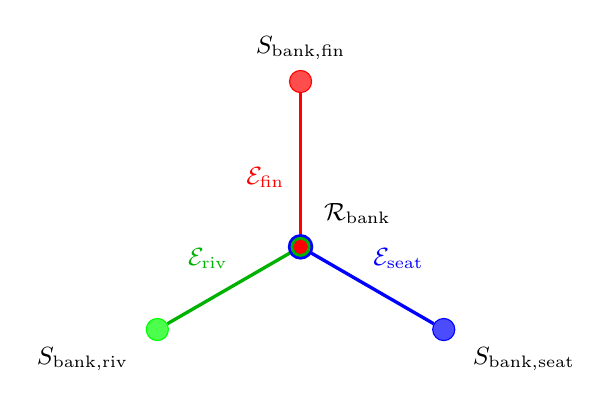
\begin{tikzpicture}[scale=0.5,
    outer/.style={circle, draw, minimum size=8pt,
                  inner sep=0pt, font=\footnotesize},
    lab/.style={font=\small}]
% central shared reference-subspace vertex
\coordinate (c) at (0,0);

\node[lab, above right=7pt] at (c)
{$\mathcal R_{\rm bank}$};

% outer sense-subspace vertices
\node[outer, red, fill=red!70,
      label={[lab]above:
      $S_{{\rm bank},{\rm fin}}$}]
      (fin) at (90:4.2cm) {};

\node[outer, green, fill=green!70,
      label={[lab, xshift=-4pt]below left:
      $S_{{\rm bank},{\rm riv}}$}]
      (riv) at (210:4.2cm) {};

\node[outer, blue, fill=blue!70,
      label={[lab, xshift=4pt]below right:
      $S_{{\rm bank},{\rm seat}}$}]
      (seat) at (330:4.2cm) {};

% hyperedges labelled by context
\draw[very thick, red] (c) --
      node[lab, left=2pt, pos=0.45]
      {$\mathcal E_{\rm fin}$} (fin);

\draw[very thick, green!70!black] (c) --
      node[lab, above left=1pt, pos=0.45]
      {$\mathcal E_{\rm riv}$} (riv);

\draw[very thick, blue] (c) --
      node[lab, above right=1pt, pos=0.45]
      {$\mathcal E_{\rm seat}$} (seat);

% central concentric disks
\filldraw[blue, very thick] (c) circle (8pt);
\filldraw[green!70!black, very thick] (c) circle (6pt);
\filldraw[red, very thick] (c) circle (4pt);
\end{tikzpicture}
\caption{%
Hypergraph schematic of context organization for the polysemous token
``bank.'' The original star geometry is retained, but its elements are now
typed as abstract hypergraph objects rather than spatial vectors. The central
vertex denotes the shared token reference subspace $\mathcal R_{\rm bank}$;
the colored outer vertices denote the complete low-dimensional sense
subspaces $S_{{\rm bank},C}\subset\mathcal R_{\rm bank}^{\perp}$, not
individual directions. Each colored spoke is the context hyperedge
$\mathcal E_C=\{\mathcal R_{\rm bank},S_{{\rm bank},C}\}$ for
$C\in\{{\rm fin},{\rm riv},{\rm seat}\}$. Each hyperedge is the
combinatorial shadow of a context projector $\Pi_{{\rm bank},C}$ or observable
$A_{{\rm bank},C}$. Because each displayed hyperedge
has two abstract vertices, it is drawn as an ordinary line; a context with
additional components would be a higher-order hyperedge incident on all of
them. The star is an incidence diagram, not a coordinate plot, and its spokes
do not denote vector directions, maps, or causal flow.
}
\label{fig:reference-subspace}
\end{figure}

\subsection{Packing sense subspaces in a shared orthogonal carrier}
\label{sec:grassmann}

The vector packing bound extends to low-dimensional subspaces.  Fix a
reference subspace $\mathcal R_t$ of rank $p$.  Its orthogonal complement has
exact dimension $d-p$.  To state the comparison simply, suppose the candidate
sense subspaces have a common local rank $q\ll d-p$.  For any fixed threshold
$\mu>2\sqrt{q/(d-p)}$, there exist many such subspaces
$S_1,\dots,S_M\subset\mathcal R_t^\perp$ satisfying
%
\begin{equation}
\label{eq:grassmann-coherence}
\opnorm{U_a\T U_b}\le \mu,\qquad a\neq b,
\end{equation}
%
where $U_a,U_b\in\R^{d\times q}$ are orthonormal basis matrices whose columns
lie in $\mathcal R_t^\perp$, and
%
\begin{equation}
\label{eq:grassmann-count}
M\ge \exp\!\bigl(c_{\mu,q}(d-p)\bigr)
\end{equation}
%
for some positive $c_{\mu,q}$.

This is a standard Grassmannian packing consequence of concentration on
Stiefel and Grassmann manifolds~\cite{szarek1982nets,conway1996packings}.
For two independent Haar-random $q$-planes, the singular values of $U\T V$
are the cosines of their principal angles. In the regime $q\ll d-p$, the
largest principal correlation is of order
$\sqrt{q/(d-p)}$~\cite{chikuse2003statistics,absil2006condition,edelman1998random}.
A union bound over sampled subspaces then gives an exponential packing.

Here $p$ and $q$ are local subspace ranks, and $M$ counts candidate sense
subspaces; none is a new global capacity dimension.  For trained
representations, the comparison assumes that the usable $d$-dimensional
carrier has already been selected or whitened.  Otherwise the Haar-random
subspace model is not a good description of activation geometry.

\subsection{Relation to dynamic contextual embeddings}
\label{sec:dynamic}

Transformers already handle polysemy dynamically. The hidden state
$h_\ell(t\mid x)$ of token $t$ at layer $\ell$ depends on context $x$.
The reference-subspace and intertwined-observable hypotheses are not
alternative hardware architectures; they are proposed organizations and
readouts of these observed trajectories.

Given a candidate reference subspace $\mathcal R_t$ and its projector $P_t$,
write
%
\begin{align}
\label{eq:layer-decomp}
h_\ell(t\mid x)
&=P_t h_\ell(t\mid x)+z_\ell(t,x),\\
z_\ell(t,x)&=(I-P_t)h_\ell(t\mid x)
\in\mathcal R_t^\perp.\nonumber
\end{align}
%
The decomposition is automatic; the hypothesis is not. It predicts that
$P_t h_\ell(t\mid x)$ tracks token identity or engagement, while
$z_\ell(t,x)$ carries most sense-disambiguating information. Sense labels
should be more separable in $\mathcal R_t^\perp$ than in the orthogonal
complements of matched control subspaces. For each sense $C$, the projected
states $z_\ell(t,x)$ should also concentrate near the low-dimensional
subspace $S_{t,C}\subset\mathcal R_t^\perp$.

Thus the critical question is not whether contextual embeddings move; they
do. It is whether their sense-relevant movement has a privileged organization
relative to a token-associated reference subspace, and whether conditional
application of $\Pi_{t,C}$ explains that movement better than matched
unstructured projectors.

\begin{table*}[ht]
\caption{Dynamic contextual embeddings versus the intertwined-observable
hypothesis.}
\label{tab:two-views}
\centering
\begin{minipage}{0.72\textwidth}
\begin{ruledtabular}
\begin{tabular}{@{}ll@{}}
Dynamic description & Intertwined-observable hypothesis \\
\colrule
Token state changes by context and layer & State is projected relative to $\mathcal R_t$ \\
Layer activation carries context & $\mathcal R_t^\perp$ contains sense variation \\
Polysemy by vector deformation & Polysemy by conditional projection $\Pi_{t,C}$ \\
Resource is depth and width & Resource is the Goldilocks bracket \\
Limit is activation bottleneck & Limit is crowding plus readout interference \\
\end{tabular}
\end{ruledtabular}
\end{minipage}
\end{table*}

% ======================================================================
\section{Attention and latent context selection}
\label{sec:attention}
% ======================================================================

A standard attention head computes
%
\begin{equation}
\label{eq:attention}
h'=\sum_j\alpha_j\nu_j,
\qquad
\alpha_j=
\frac{\exp(q_{\rm att}\T k_{{\rm att},j}/\sqrt{d_{\rm head}})}
{\sum_{j'}\exp(q_{\rm att}\T k_{{\rm att},j'}/\sqrt{d_{\rm head}})} .
\end{equation}
%
$q_{\rm att},k_{{\rm att},j}\in\R^{d_{\rm head}}$ are the query and key
vectors of that head.  The local head width $d_{\rm head}$ is an architectural
quantity, not the usable carrier dimension $d$ in the Goldilocks calculation.
Keys and values are produced by different learned maps, so value vectors
are not generally coefficients of a dual basis for the key vectors.
Attention is therefore not literal basis reconstruction.

The useful analogy is softer. Attention routes information: it amplifies
some contextual directions and suppresses others. In the terminology of
Sec.~\ref{sec:reference}, this resembles context-dependent subspace
selection. A literal basis-reconstruction interpretation would require
additional constraints, such as approximately Parseval keys and values
implementing the corresponding dual reconstruction. We do not assume this.

A compact latent-variable version is
%
\begin{equation}
\label{eq:latent}
p(y\mid x,t)=\sum_C p(y\mid x,t,C)\,p(C\mid x,t),
\end{equation}
%
where $t$ is the token being disambiguated, $y$ is a possible output token,
and $C$ indexes candidate sense contexts. One may model
%
\begin{equation}
\label{eq:context-temp}
p(C\mid x,t)=
\frac{\exp(s_{t,C}(x)/T)}
{\sum_{C'}\exp(s_{t,C'}(x)/T)} ,
\end{equation}
%
with $s_{t,C}$ the gated score of Eq.~\eqref{eq:sense-score}. This is not
a claim about the literal implementation of decoding in current LLMs:
standard temperature acts on token logits, not on explicit latent
sense labels. The point is only that ambiguity can be represented as a
distribution over possible sense contexts rather than as a single fixed
interpretation.

The same weights provide a soft implementation of the intertwined-observable
construction:
%
\begin{equation}
\label{eq:soft-observable-embedding}
\bar h_t(x)
=\sum_C p(C\mid x,t)\,h_{t,C}(x)
=\sum_C p(C\mid x,t)\,\Pi_{t,C}h(x).
\end{equation}
%
Hard selection uses $C^*$ from Eq.~\eqref{eq:selected-sense}; soft selection
uses Eq.~\eqref{eq:soft-observable-embedding}.  Attention may supply the
routing signal $p(C\mid x,t)$, but the structured projectors or observables
are an additional model component and should not be identified with standard
attention weights without empirical evidence.

% ======================================================================
\section{Discussion}
\label{sec:discussion}
% ======================================================================

The geometric proposal is the capacity/accessibility distinction sharpened
into the Goldilocks estimate~\eqref{eq:gold-simple}.  The intertwined-observable
model is one possible contextual organization within that bracket, not a
consequence of concentration geometry.

\subsection{Relation to superposition and sparse autoencoders}
\label{sec:superposition}

The superposition hypothesis holds that neural networks represent more
features than they have neurons by packing features into nearly
orthogonal directions~\cite{elhage2022superposition,bricken2023monosemanticity}. The concentration
estimate~\eqref{eq:overlap} gives the kinetic side of that picture:
many directions can coexist. Equation~\eqref{eq:sint} gives the
epistemic side: many jointly active features create interference of
scale $\sqrt{k/d}$. Sparsity is therefore not an implementation
detail; it is necessary for readout.

Sparse autoencoders (SAEs) give a concrete empirical interface. They
approximate layer activations as sparse expansions over learned decoder
directions, making the $w_i$ of Eq.~\eqref{eq:hidden} measurable
objects rather than hypothetical features. Recent work has scaled SAEs,
studied SAE feature geometry, and automated interpretation of large
numbers of latents~\cite{gao2025scaling,li2025geometry,paulo2025automatically,shu2025survey}. In the
present framework, SAE decoder directions can test the
capacity/accessibility prediction, while sense-conditioned SAE
activation clusters can test the stronger reference-subspace hypothesis.

\subsection{A coactivation-weighted capacity limit}
\label{sec:capacity-limit}

The active-set size $k$ is a crude summary. A more refined description
uses the coactivation graph
%
\begin{equation}
\label{eq:coactivation}
A_{ij}=\Prob(i,j\text{ active}).
\end{equation}
%
If active amplitudes have, conditional on coactivation, zero mean and
pairwise uncorrelated signs, then cross terms cancel in expectation and
feature $j$ contributes to the readout variance of feature $i$ in
proportion to
$\E[x_j^2\mid i,j\text{ active}](w_i\T w_j)^2$. Absorbing amplitude
variance and feature importance into coefficients $b_i,b_j$ gives
%
\begin{equation}
\label{eq:int-energy}
\Eint=
\sum_{i\neq j}
A_{ij}b_i b_j (w_i\T w_j)^2 .
\end{equation}
%
Frequently coactive features are therefore pressured toward
orthogonality. Rarely coactive or mutually exclusive features are much
less constrained and may share directions or even become approximately
antipodal if nonlinear readout makes this useful. The relevant object
is not just the number of features, but the weighted coactivation graph.

\subsection{Limitations}
\label{sec:limitations}

The framework can fail in several ways.

First, the Goldilocks bracket is a random-code estimate, not a
model-independent hard boundary. Equation~\eqref{eq:max-overlap} assumes
independent isotropic directions. Learned dictionaries can beat or
underperform that null model. The bracket is informative only after the
usable exact dimension $d$, dictionary count $\Nq$, and tolerated overlap
$\varepsilon$ have been specified. The active count $k$ belongs to the
separate readout test.

Second, the nominal layer width need not equal the usable exact dimension
$d$. Contextual embeddings can be anisotropic, and the occupied carrier can
vary strongly by layer and training regime
\cite{ethayarajh2019,gao2019representation,mu2018allbutthetop,razzhigaev2024shape}. Whitening and
related postprocessing can partially restore isotropic geometry
\cite{gao2019representation,mu2018allbutthetop,su2021whitening}. At the same time, anisotropy should not
be treated as an automatic or universal property of all Transformer
representations~\cite{machina2024anisotropy}. The rule used to select or
whiten a $d$-dimensional usable carrier must therefore be reported. We do not
introduce a separate $d_{\rm eff}$.

Third, the spanning matrix $U_{t,C}$ needs to be well-conditioned. If
$\rho$ in Eq.~\eqref{eq:rho-stable} is close to one, its dual amplifies
readout noise.

Fourth, the reference-subspace pattern may simply be descriptively wrong. Trained
models may represent polysemy without any preferred token-associated
direction or subspace. In that case the capacity/accessibility
account may still hold, but the reference-subspace hypothesis fails.

Fifth, the law $\sint\sim\sqrt{k/d}$ assumes random-like
incoherent directions and weakly correlated signs or amplitudes.
Learned networks may improve on this by orthogonalizing frequently
coactive features, or worsen it through anisotropy and correlated
errors. The law is a scaling principle, not a universal equality.

Finally, the operator model has choices: the candidate reference subspace
$\mathcal R_t$, the gate, the selector, the sense-subspace dimension, and the
spectra in Eq.~\eqref{eq:context-observable}.  The eigenvalues are not
identified by the subspaces alone. These choices must be fixed or learned
under held-out evaluation; otherwise the framework risks describing whatever
geometry is found after the fact.

\subsection{Empirical predictions}
\label{sec:predictions}

The key empirical task is to separate the geometric bracket from the stronger
reference-subspace and intertwined-observable claims.

{Claim G: a calibrated Goldilocks regime.}
For a prespecified overlap tolerance $\varepsilon$, a useful overcomplete
representation should have $\Nq>d$ while its measured maximum overlap remains
compatible with Eq.~\eqref{eq:max-overlap}. Its accessibility should be tested
separately against the active-set scaling in Eq.~\eqref{eq:sint}.

{Claim A: privileged token reference subspace.}
For a polysemous token $t$, there exists a privileged token-associated
subspace $\mathcal R_t$ such that sense-relevant variation is better
exposed in $\mathcal R_t^\perp$ than in the orthogonal complements of
matched control subspaces of the same dimension.

{Claim B: low-dimensional sense subspaces.}
Within $\mathcal R_t^\perp$,
sense-conditioned states concentrate near low-dimensional subspaces
with small cross-sense coherence.

{Claim C: intertwined context operators.}
Context projectors $\Pi_{t,C}$ share $P_t$, differ on
$\mathcal R_t^\perp$, and improve held-out contextual prediction or
compression relative to dimension-matched unstructured projectors.  Where
contexts are operationally incompatible, their fitted commutator should be
nonzero and sequential projection should be order-sensitive.

These claims can fail independently. Claim G concerns the global dictionary
and active-set geometry. Claim A can hold while sense
information remains high-dimensional. Claim B can hold relative to some
non-token-associated subspace, in which case Claim A fails. Claims A and B can
hold even if the operator constraint in Claim C adds no predictive value.

The following tests separate the possibilities.

\begin{enumerate}
\item \emph{Goldilocks calibration test.}
Choose the usable carrier by a declared spectral threshold or whitening rule
and report its exact basis size $d$. Count a prespecified dictionary of $\Nq$
feature directions, measure its maximum overlap, and estimate active-set size
$k$. Compare the observed crowding and recovery behavior with
Eqs.~\eqref{eq:max-overlap} and~\eqref{eq:sint}. The comparison must include
isotropic random dictionaries and trained, coactivation-matched controls.

\item \emph{Reference-subspace test.}
For a polysemous token, choose candidate reference subspaces generated
by the normalized static input embedding, mean contextual embedding,
learned token-specific directions, or a low-dimensional combination of
these. Project layer states as in Eq.~\eqref{eq:layer-decomp}. Sense labels
should be better separated in $\mathcal R_t^\perp$ than in orthogonal
complements of random, frequency-matched, or layer-matched control
subspaces of the same dimension. The statistic may be classification accuracy or
mutual information with sense labels, assessed by permutation over
sense labels and bootstrap over token instances.

\item \emph{Operational subspace test.}
For each sense $s$, collect projected states
$z_\ell(t,x)\in\mathcal R_t^\perp$ and estimate a low-rank subspace by PCA or
probabilistic factor analysis. With $U_{t,s}$ the first $q$ principal
directions for sense $s$, measure cross-sense coherence
$\opnorm{U_{t,s}\T U_{t,s'}}$. True sense labels should yield lower
cross-sense coherence than shuffled labels and stronger separation than
matched control reference subspaces.

\item \emph{Gated-readout test.}
Linear probes trained on $z_\ell(t,x)$ should perform comparably to
probes trained on the full state $h_\ell(t\mid x)$, while probes
restricted to the reference component $P_t h_\ell(t\mid x)$ should perform
near chance on sense classification.

\item \emph{Intertwined-observable test.}
Fit $P_t$ and $B_{t,C}$ on training contexts, construct $\Pi_{t,C}$ and
$A_{t,C}$, and evaluate Eq.~\eqref{eq:observable-embedding} on held-out
instances. Compare against unconstrained low-rank projectors, mixture-of-
experts probes with the same parameter count, and shuffled context labels.
Report $\opnorm{[\Pi_{t,C},\Pi_{t,C'}]}$ and test whether reversing sequential
context projections changes predictions where the model claims contextual
incompatibility.

\item \emph{Overlap-distribution test.}
If a representation exploits quasi-dimensionality, pairwise inner
products among token embeddings or SAE feature directions should
concentrate near zero with variance $\sim1/d$ after the usable carrier has
been selected. Deviations quantify anisotropy or learned alignment not
captured by the random null model.

\item \emph{Synthetic concurrency degradation.}
At a fixed layer, inject controlled superpositions
%
\begin{equation}
h_k=h_0+\lambda\sum_{j=1}^k x_j w_j,
\end{equation}
%
using directions $w_j$ obtained independently, for example from SAE
decoder directions or frozen linear probes. As $k$ increases, readout
should degrade smoothly on the scale $\sqrt{k/d}$ for random-like
directions, with weaker degradation for feature sets that training has
orthogonalized.

\item \emph{Coactivation-dependent geometry.}
Frequently coactive features should show reduced mutual coherence
relative to rarely coactive features. This tests the broader
capacity/accessibility framework through Eq.~\eqref{eq:int-energy},
independently of the reference-subspace hypothesis.
\end{enumerate}

\subsection{Scope of the quantum analogy}
\label{sec:quantum}

The analogy to quantum contextuality is structural and limited. Both settings
can describe alternatives by observables with context-dependent eigenspaces.
In the proposed construction, the operators $A_{t,C}$ intertwine because they
share the spectral projector $P_t$; their complementary sense sectors may
yield nonzero commutators.  The hyperedges in
Fig.~\ref{fig:reference-subspace} record only this incidence pattern, whereas
Eqs.~\eqref{eq:context-projector}--\eqref{eq:context-observable} supply its
operator realization.  A basis is a set of vectors, a subspace is their span,
and an observable is an operator with a spectral decomposition; these objects
are not interchangeable.

Quantum contextuality has the force of no-go theorems such as
Kochen--Specker~\cite{specker-60,kochen1}; no analogous theorem is claimed
here for semantic embeddings.  Real symmetric matrices can be noncommuting
while still being stored and evaluated on an ordinary classical computer.
Thus the operator construction is quantum-inspired, but noncommutativity by
itself supplies neither Born probabilities nor physical quantumness.

Three levels of analysis should not be conflated.
%
\begin{enumerate}
\item \emph{Classical high-dimensional representation.}
A present-day Transformer carries real-valued hidden states through
attention, nonlinear feed-forward maps, residual connections, and
normalization.  Concentration, quasi-orthogonality, feature superposition,
dynamic embeddings, and finite readout are all available at this level.
None requires quantum probability or quantum hardware.

\item \emph{Quantum-like semantic or contextual formalism.}
States, contexts, bases, interference terms, noncommuting questions, or
measurement-like updates may be used as an abstract model of meaning even
when the implementation remains classical.  The relevant issue is not the
vocabulary but whether this extra structure improves compression,
explanation, or prediction relative to an ordinary contextual embedding
model.

\item \emph{Genuine quantum machine learning or quantum attention.}
Here semantic states would be encoded in qubits or other physical quantum
degrees of freedom, intermediate evolution would be unitary, phase would
affect interference, and measurement would follow quantum probability.  A
standard Transformer does none of these things.
\end{enumerate}
%

The Goldilocks bracket belongs entirely to the first level: it is a claim
about classical high-dimensional geometry.  The shared-subspace hypothesis
is likewise testable in a classical model.  The intertwined operators and
their order-sensitive projections belong to the second level because they
make the quantum-inspired comparison explicit and implementable.  Their
scientific value depends on the discriminative test in
Sec.~\ref{sec:predictions}: they must improve prediction, compression, or
explanation relative to equally expressive classical baselines. Even a
positive result would support a useful quantum-like formalism, not physical
quantum computation; phase-sensitive dynamics and Born-rule measurement are
still absent.

The dimension of $\mathcal R_t$ is also explicit. In Hilbert-space quantum
logic, different contexts can share one observable, as in the familiar
tripod-like case, or several observables; a four-dimensional example has
two contexts with two common observables~\cite{svozil:040102}. The semantic
analogue is $\dim(\mathcal R_t)=p$: $p=1$ is the simplest case, while
$p>1$ permits several token-associated reference directions. In every case,
sense-specific information is hypothesized to occupy subspaces of
$\mathcal R_t^\perp$.

% ======================================================================
\section{Conclusion}
\label{sec:conclusion}
% ======================================================================

Useful quasi-dimensionality is governed by two global counts.  The exact
dimension $d$ is the size of an orthonormal basis of the usable carrier.  The
quasi-dimensional count $\Nq$ is the number of approximately orthogonal
semantic directions represented in it.  Only $d$ is literally a vector-space
dimension; $\Nq$ is the size of an overcomplete semantic dictionary.  Their
plain-language Goldilocks relation is
%
\begin{equation}
\label{eq:summary}
\boxed{
d<\Nq\ \lesssim\ \exp\!\left(\frac{d\varepsilon^2}{4}\right)
},
\end{equation}
%
where $\varepsilon$ is the largest tolerable overlap.  Below the left edge,
an exactly orthogonal assignment remains possible.  Above the right edge,
random-like directions become too crowded for that overlap criterion.

This capacity statement is distinct from accessibility.  If $k$ directions
are active together, their interference scales as $\sqrt{k/d}$.  The symbol
$k$ is an active-set count, not a third dimension.  Thus there is no universal
``right dimension'' independent of the dictionary, tolerated overlap, and
readout task.  For illustration, $d=4096$ and $\varepsilon=0.10$ give
$4096<\Nq\lesssim2.8\times10^4$ under the isotropic random-code estimate;
$k=64$ gives an interference scale of $0.125$.  These numbers demonstrate the
calculation but are not LLM constants.

The second central construction implements intertwined contexts.  For a
polysemous token, the context observables $A_{t,C}$ share the spectral
projector $P_t$ associated with token identity and differ on sense subspaces
of $\mathcal R_t^\perp$.  Their projectors $\Pi_{t,C}$ can fail to commute,
and conditional projection
$h_{t,C}=\Pi_{t,C}h$ supplies a context-specific embedding.  A soft selector
forms the mixture in Eq.~\eqref{eq:soft-observable-embedding}.  The ``bank''
schematic displays the financial, river-edge, and seat/bench contexts; the
aircraft-banking sense is a possible fourth hyperedge rather than a replacement
for the intended seat association.

These two ideas have different evidential status.  The Goldilocks bracket is
a classical geometric null model whose parameters can be measured directly.
The shared reference subspace, the noncommuting context operators, and their
predictive usefulness are stronger hypotheses.  They must outperform
dimension- and parameter-matched classical baselines on held-out data.  A
failure of the operator model would leave the capacity/interference bracket
intact; a failure of the random-code bracket would reveal learned structure,
anisotropy, or nonlinear readout not captured by the null model.

Finally, the operator construction is quantum-inspired, not a claim that a
Transformer is a quantum device.  It uses real matrices on classical hardware
and introduces no Born rule, unitary dynamics, or physical measurement.
Its value lies in whether shared spectral projectors, incompatible context
operators, and order-sensitive conditional embeddings provide a more compact
or predictive account of polysemy.  That question is discriminative and
falsifiable; the vocabulary of quantum contextuality is useful only to the
extent that the proposed tests answer it positively.

\begin{acknowledgments}
OpenAI Codex (GPT-5) was used to assist with literature organization, \LaTeX{}
editing, and checks of derivations.  The authors specified the scientific
direction and prompts; model output retained in the manuscript was checked
against the cited sources and explicit calculations.  The authors accept full
responsibility for the final text.

This research was funded in part by the Austrian
Science Fund (FWF), Grant digital object identifier (DOI)
\href{https://doi.org/10.55776/PIN5424624}{10.55776/PIN5424624}.
The author acknowledges FWF and TU Wien Bibliothek for financial support through its
Open Access Funding Programme.

The authors declare no conflict of interest.
\end{acknowledgments}

\bibliography{svozil}

\end{document}
